\documentclass{article}
\usepackage{amsmath}
\usepackage[dvipdfmx]{graphicx}

\title{タイトル}
\author{著者}
\date{日付}

\begin{document}
    \maketitle
    \newpage

    \section{Hello World}
    Hello!
    \subsection{数式表現}
    \begin{equation}
        e^{i\pi}+1=0
    \end{equation}

    \subsection{箇条書き}
    % 箇条書きの場所
    \begin{itemize}
        \item りんご
        \item ごりら
        \item らっぱ
    \end{itemize}

    \subsection{表}
    % 表の場所
    \begin{table}[htbp]
        \centering
        \caption{サンプル表}
        \begin{tabular}{|l|c|r|}
            \hline
            左揃え & 中央揃え & 右揃え \\
            \hline
            $\alpha$ & $\beta$ & $\gamma$ \\
            \hline
            alpha & beta & gamma \\
            \hline
        \end{tabular}
    \end{table}

    \subsection{画像}
    % 画像の場所
    \begin{figure}
        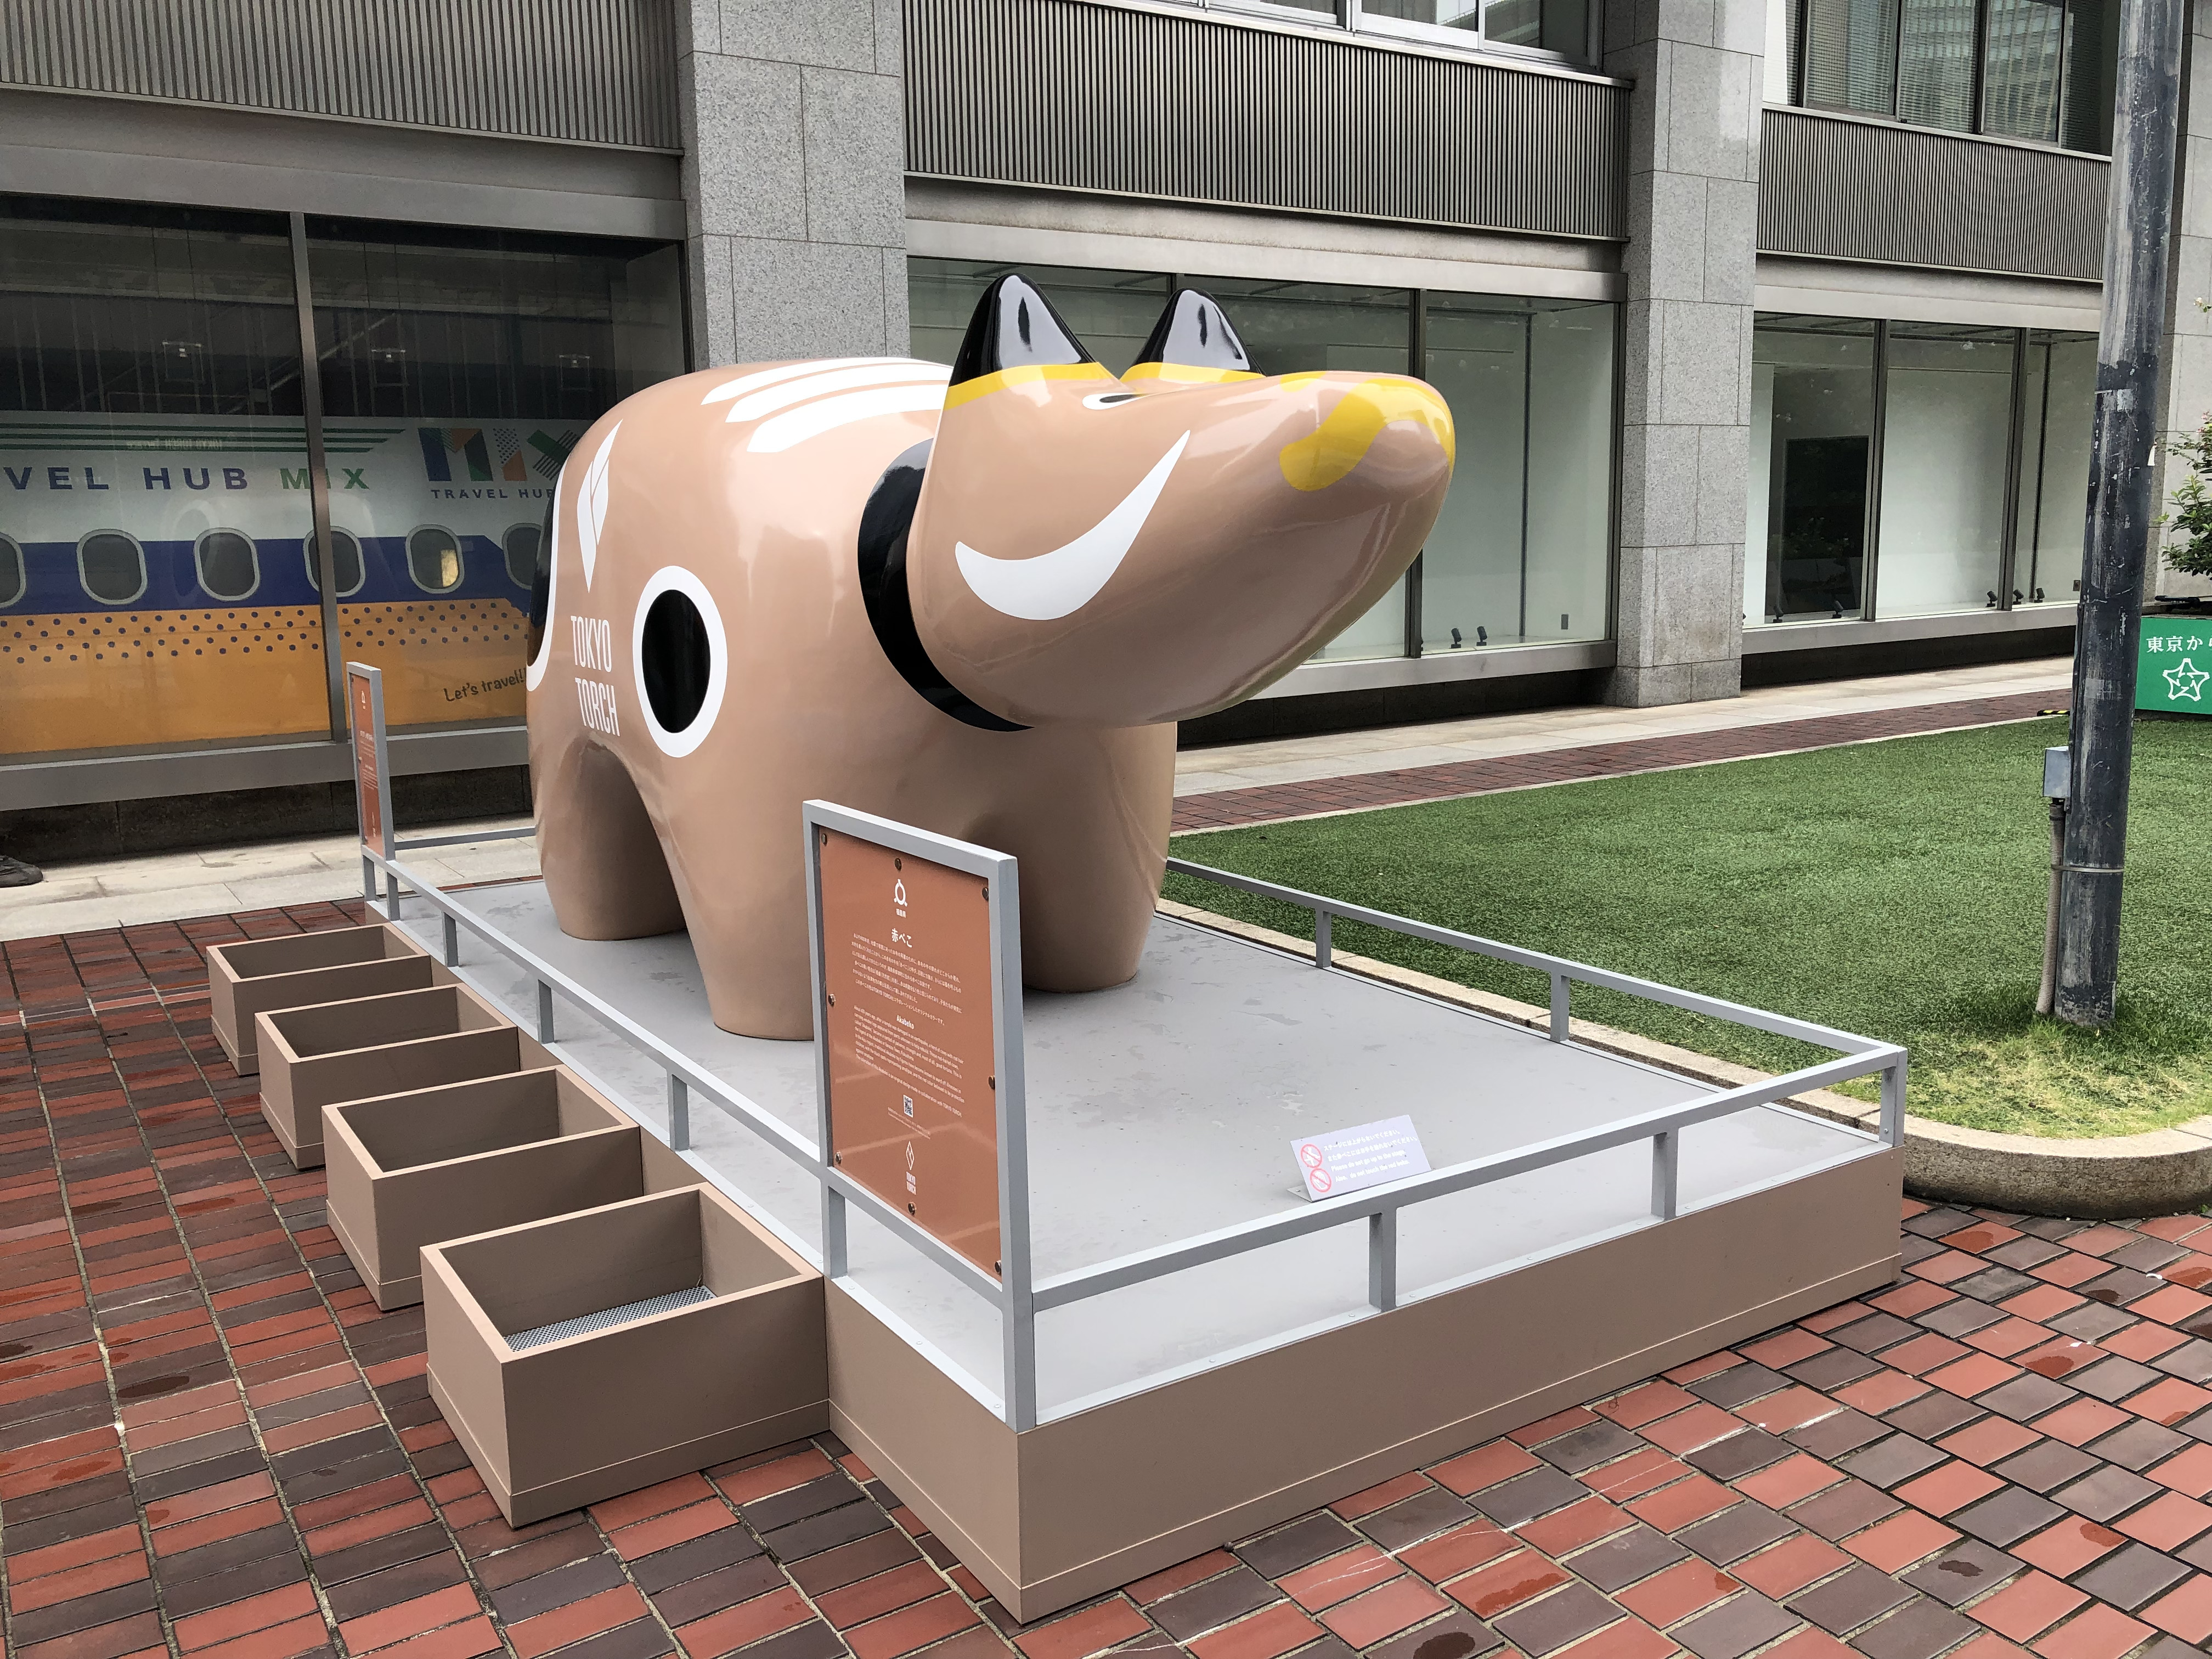
\includegraphics[width=\linewidth]{akabeko.jpg}
        \caption{東京駅前の赤べこ}        
    \end{figure}
\end{document}
